% podpunkt A: w tekście zamiast nazwy rysunku jest "??"
\documentclass{article}

\usepackage{polski}
\usepackage{amsmath,amsfonts,stmaryrd,amssymb} 
\usepackage[framemethod=tikz]{mdframed}
\usepackage[utf8]{inputenc}
\usepackage{geometry} 
\usepackage{titlesec}

\usepackage{graphicx}
\usepackage{caption}
\usepackage{subcaption}
\captionsetup{compatibility=false}
\usepackage{epstopdf}

\geometry{
	paper=a4paper,
	top=2.5cm, 
	bottom=3cm,
	left=2.5cm,
	right=2.5cm,
	headheight=14pt,
	footskip=1.5cm,
	headsep=1.2cm,
}

\titlelabel{\thetitle.\quad}

\pagenumbering{gobble}

\title{
	\textbf{Pracownia z analizy numerycznej}\\[8pt]
	\large{Sprawozdanie do zadania \textbf{P2.19}\\
	Prowadzący: dr hab. prof. Paweł Woźny}}

\author{\large{Martyna Firgolska, Michał Dymowski}}

\date{\large{Wrocław, \today}}

\newtheorem{theorem}{Twierdzenie}



\begin{document}

\maketitle 

\section*{Wstęp}
Liczenie wartości całki oznaczonej jest istotnym zagadnieniem matematycznym wykorzystywanym w fizyce i innych naukach ścisłych. Dla niektórych funkcji $f$ jesteśmy w stanie łatwo znaleźć funkcję pierwotną $F$ czyli taką, że $F' = f$. Jeśli umiemy w łatwy sposób obliczyć wartość $F$ w danym punkcie to możemy obliczyć wartość całki oznaczonej: $\int_a^b f(x) dx = F(b) - F(a) $. Niestety dla niektórych funkcji $f$ znalezienie $F$ i jej wartości dla danych punktów nie jest łatwe. Z tego powodu chcielibyśmy w jakiś sposób przybliżać wartości całek oznaczonych obliczając wartości znanej nam funkcji $f$. Metody numeryczne, które obliczają te przybliżone wartości nazywamy kwadraturami. Poniższe sprawozdanie dotyczy porównania dokładności różnych kwadratur dla niżej opisanych funkcji.
\section*{Badane funkcje}
W tym sprawozdaniu zbadamy skuteczność różnych metod numerycznych w obliczaniu przybliżonych wartości całek dla funkcji $C = \frac{cos(x)}{\sqrt{x}}$ i $S = \frac{sin(x)}{\sqrt{x}}$ na przedziale $[0, 1]$. Całkowane funkcje nie są zdefiniowane w $0$, na potrzeby obliczeń przyjmiemy, że wartości tych funkcji w $0$ są równe $0$. 

\begin{equation}
I_C = \int_0^1 \frac{cos(x)}{\sqrt{x}} dx \approx 1.8090484758005441629...
\end{equation}
\begin{equation}
I_S = \int_0^1 \frac{sin(x)}{\sqrt{x}} dx \approx 0.6205366034467622036...
\end{equation}
%\begin{figure}

\begin{figure}[ht]
    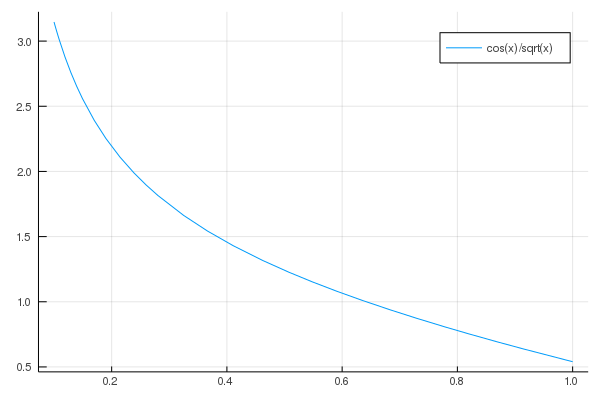
\includegraphics[scale=0.5]{WykresC.png}
    \label{wykresC}
\end{figure}
\begin{figure}[ht]
    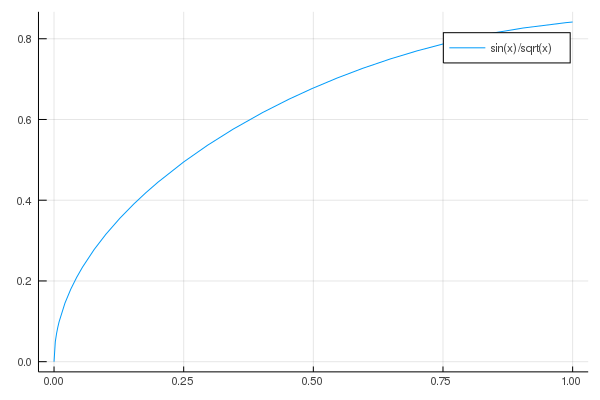
\includegraphics[scale=0.5]{WykresS.png}
    \label{WykresS}
\end{figure}
%\end{figure}
Przyjrzyjmy się wykresom badanych funkcji na podanym przedziale. Zauważamy, że $C$ w zerze rozbiega do nieskończoności, a $S$ w zerze zbiega do $0$. Reczywiście obliczenie granic daje wyniki zgodne z wykresami funkcji:
\begin{equation}
\lim_{x\to 0}  \frac{cos(x)}{\sqrt{x}} = \lim_{x\to 0} \frac{cos(0)}{\sqrt{x}} = +\infty
\end{equation}
\begin{equation}
\lim_{x\to 0}  \frac{sin(x)}{\sqrt{x}} = \lim_{x\to 0}  \frac{sin(x)}{x} \sqrt{x} = 0
\end{equation}
Na podstawie tej informacji możemy przypuszczać, że obliczenie całki $I_S$ będzie łatwiejsze niż obliczenie $I_C$, ponieważ $S$ jest ograniczona, a jej wartość w $0$ zgadza się z jej granicą w tym punkcie. $C$ jest nieograniczona i w zerze przyjmuje $0$, ale jej granica w tym punkcie wynosi $+\infty$ zatem obliczenie całki w okolicy $0$ może być niedokładne.\\
Możemy zmienić postać całek $I_C$ i $I_S$ za pomocą podstawienia $x=t^2$ Wtedy:
\begin{equation}
I_C = \int_0^1 \frac{cos(t^2)}{\sqrt{t^2}} 2tdt = \int_0^1 2cos(t^2)
\end{equation}
\begin{equation}
I_S = \int_0^1 \frac{sin(t^2)}{\sqrt{t^2}} 2tdt = \int_0^1 2sin(t^2)
\end{equation}
Otrzymujemy w ten sposób nowe funkcje pod całką $Snew(x) = 2sin(x^2)$ i $Cnew(x) = 2cos(x^2)$. Nowe funkcje mają określone wartości dla wszystkich punktach z przedziału $[0,1]$ i obie funkcje są ograniczone, więc nie mamy takiego problemu jak przy funkcji $C$.
\begin{figure}[ht]
    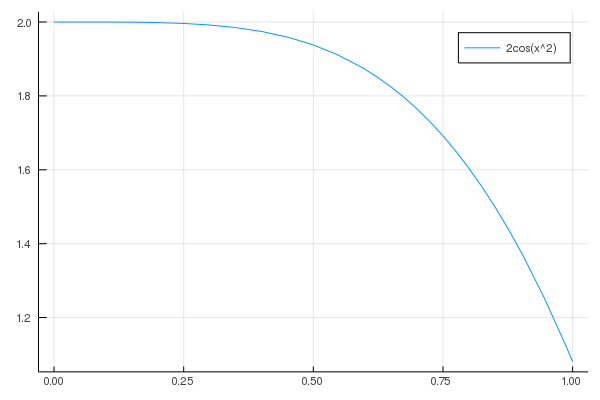
\includegraphics[scale=0.5]{WykresCnew.png}
    \label{wykresCnew}
\end{figure}
\begin{figure}[ht]
    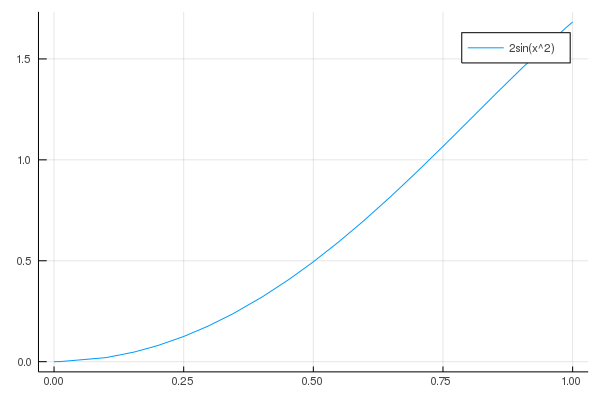
\includegraphics[scale=0.5]{WykresSnew.png}
    \label{WykresSnew}
\end{figure}
\section*{Metoda trapezów}
Metoda trapezów jest kwadraturą wyrażoną wzorem: 
\begin{equation}
\int_a^b f(x) dx \approx \frac{1}{2}(b-a) (f(a)+f(b))
\end{equation}
Rozumowanie użyte w tej metodzie jest następujące: skoro nie potrafimy łatwo obliczyć całki funkcji $f(x)$ to zastąpmy ją podobną funkcją, którą potrafimy zcałkować - wielomianem. Stosujemy więc interpolację (np. korzystając z wzoru Lagrange'a) i liczymy całkę z obliczonego wielomianu interpolacyjnego. 
\begin{equation}
w(x) = \sum_{i=0}^n f(x_i)l_i(x)
\end{equation}
gdzie 
\begin{equation}
 l_i(x) = \prod ^n_{j=0, j\neq i} \frac{x-x_j}{x_i-x_j} 
\end{equation}
\begin{equation}
\int_a^b f(x) dx \approx \int_a^b w(x) dx =  \sum_{i=0}^n f(x_i)\int_a^bl_i(x)
\end{equation}
Jeśli węzłami interpolacji będą punkty postaci $x_i = a+ \frac{b-a}{n} $ to powyższy wzór nazywamy wzorem Newtona-Cotesa. Dla $n=1$ czyli interpolując $f$ w 2 punktach: $x_0=a$ i $x_1=b$ otrzymujemy wyżej wspomniany wzór trapezów.\\
Zauważmy, że ta kwadratura jest dokładna dla $f$, które są wielomianami co najwyżej pierwszego stopnia. Można udowodnić, że błąd metody trapezów wynosi:
\begin{equation}
R = -\frac{1}{12}(b-a)^3f''(\xi)
\end{equation}
gdzie $\xi \in (a, b)$.
Błąd jest więc zależny od długości przedziału całkowania. Aby uzyskać dokładniejszy wynik możemy podzielić przedział $(a, b)$ na mniejsze przedziały, na przykład na $n$ przedziałów długości $h=\frac{(b-a)}{n}$, i zastosować na każdym z nich wzór trapezów. W ten sposób otrzymujemy złożony wzór trapezów
\begin{equation}
\int_a^b f(x) dx \approx \frac{1}{2} h (f(a) + 2\sum_{i=1} ^{n-1} f(a+ih) +f(b))
\end{equation}
Którego błąd wynosi:
\begin{equation}
R = -\frac{1}{12n^2}(b-a)^3f''(\xi)
\end{equation}
gdzie $\xi \in (a, b)$.
Metodę nazywamy metodą trapezów, ponieważ geometrycznie możemy myśleć o tym że przybliżamy pole pod wykresem (całkę) trapezami o wierzchołkach w punktach $ (a, 0), (a, f(a)), (b, 0), (b, f(b)) $.
\subsection*{Wyniki obliczania całek za pomocą złożonego wzoru trapezów}
\begin{tabular}{|c|c|c|} \hline
liczba przedziałów & $I_C$ & $I_S$ \\ \hline \hline
100 & 1.6677256034277628 & 0.6288262828757042 \\ \hline
200 & 1.7082394599682968 & 0.6246912988653139 \\ \hline
300 & 1.726399997150005  & 0.6233107905275299 \\ \hline
400 & 1.7372928699596446 & 0.6226195323389588 \\ \hline
500 & 1.7447564299910763 & 0.6222043082298286 \\ \hline
600 & 1.750281758632448  & 0.6219272438774593 \\ \hline
700 & 1.7545855714753669 & 0.6217291960934527 \\ \hline
800 & 1.7580609258924103 & 0.6215805696160139 \\ \hline
900 & 1.7609438155984576 & 0.6214649112045778 \\ \hline
1000& 1.7633856545771385 & 0.6213723429157811 \\ \hline
\end{tabular}\\
\\
Wyniki otrzymane za pomocą metody trapezów są coraz lepsze wraz ze wzrostem $n$. Zauważamy jednak, że polepszenie wyniku kosztem zwiększenia $n$ (co wiąże się ze zwiększeniem ilości obliczeń - czyli dłuższym obliczaniem wyniku i większymi błędami wynikającymi z zaokrągleń liczb) jest niewielkie. Jak widzimy na rysunku \ref{wykresA} logarytmy błędu maleją dość wolno. Logarytmy dziesiętne błędu oznaczają ile miejsc po przecinku wyniku jest dokładnych. Widzimy więc że w przypadku $I_C$ mamy ok. 1 cyfrę dokładną, a w przypadku $I_S$ mamy około 2 doładne cyfry po przecinku. Zauważamy również, że metoda trapezów gorzej radzi sobie z funkcją $C$ niż z $S$.
\begin{figure}[ht]
    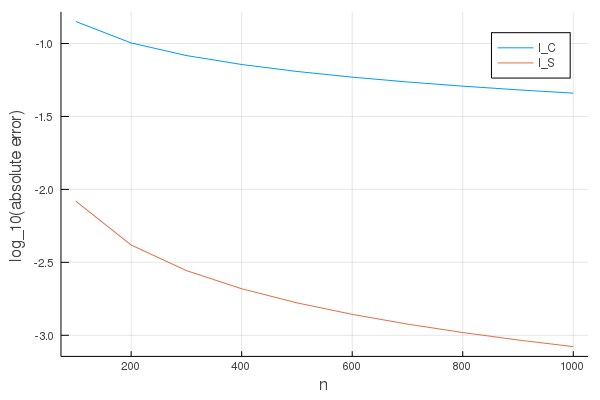
\includegraphics[scale=0.5]{WykresAlogabsolute.png}
    \label{wykresA}
    \caption{logarytm z błędu bezwzględnego obliczenia całek $I_C$ i $I_S$ wzorem złożonym trapezów dla różnych n}
\end{figure}
\section*{Modyfikacja złożonego wzoru trapezów}
Sprawdzamy czy na dokładność otrzymanego wyniku wpłynie zmiana sposobu całkowania danych funkcji w pewnym otoczeniu punktu 0, a poza tym otoczeniem stosujemy złożony wzór trapezów. Do całkowania na przedziale $[0,h]$ dla małych wartośći $h$ stosujemy odpowiednio przekształconą tożsamość \[
	\int_0^1 x^{-1/2}f(x) dx \approx \frac{4}{3}f(0)+\frac{2}{3}f(1), \]
otrzymując \[
	I_C = \int_0^1 \frac{\cos{x}}{\sqrt{x}} dx = \int_h^1 \frac{\cos{x}}{\sqrt{x}}dx + \int_0^h \frac{\cos{x}}{\sqrt{x}} dx \approx \int_h^1 \frac{\cos{x}}{\sqrt{x}}dx + \frac{2\sqrt{h}}{3}(2\cos{0}+\cos{h}) \]
\[
	I_S = \int_0^1 \frac{\sin{x}}{\sqrt{x}} dx \approx \int_h^1 \frac{\sin{x}}{\sqrt{x}}dx + \frac{2\sqrt{h}}{3}(2\sin{0}+\sin{h}) \]
\subsection*{Wyniki dla zmodyfikowanej metody}
Poniższy wykres przedstawia wyniki dwóch sposobów wyboru długości $h$ przedziału, dla którego nie używamy złożonej metody trapezów. W pierwszym przypadku stale $h=$ 2e-10 niezależnie od ilości węzłów użytych w złożonej metodzie trapezów (krzywe $IS,IC$ na wykresie). W drugim przypadku kładziemy $h=\frac{1}{n}$, gdzie $n$ jest liczbą węzłów używanych w obecnym kroku w złożonej metodzie trapezów (krzywe $IS2,IC2$).


\begin{figure}[ht]
    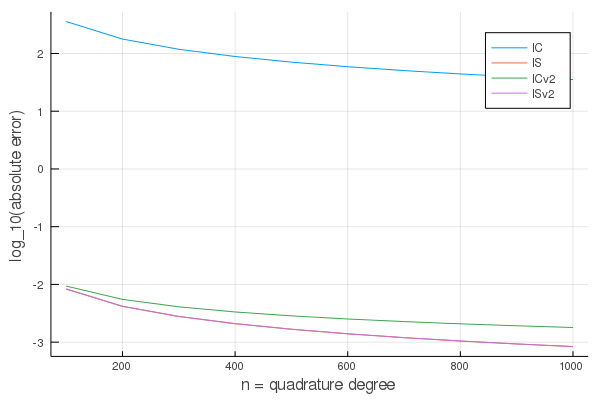
\includegraphics[scale=0.5]{WykresBlogabsolute.png}
    \label{wykresB}
\end{figure}

Krzywe $IS$ i $IS2$ pokrywają się. Wyniki obliczenia całki $I_S$ nie różnią się ilością cyfr dokładnych od wyników uzyskanych przy pomocy złożonego wzoru trapezów, natomiast w przypadku całki $I_C$ zastosowanie metody 2. daje 2-3 cyfry dokładne (złożony wzór trapezów dawał tylko jedną). Tak duża róźnica w dokładności otrzymanego wyniku pomiędzy podejściem 1. i 2. dla całki $I_C$ oraz $n=1000$ węzłów jest niespodziewana, ponieważ chociaż w metodzie 2. przedział na którym nie używamy metody trapezów jest dłuższy niż w metodzie 1. to w tym przypadku różnica długości tych przedziałów jest rzędu 2e-16, a więc jest znacznie mniejsza niż różnica uzyskanych wyników, a przecież całkujemy funkcje o wartościach w przedziale $[-1,1]$.

\section*{Metoda trapezów po podstawieniu $x=t^2$}
Po wykonaniu podstawień (5) i (6) otrzymujemy nowe funkcje podcałkowe $2\sin{x^2}$ i $2\cos{x^2}$ pozbawione osobliwości w punkcie 0. Można spodziewać się, że zastosowanie złożonego wzoru trapezów dla funkcji ciągłych na całym przedziale całkowania da lepsze wyniki, ponieważ skoro nasz przedział jest ograniczony, to funkcje które całkujemy są na nim jednostajnie ciągłe.

\newpage

\begin{figure}[ht]
    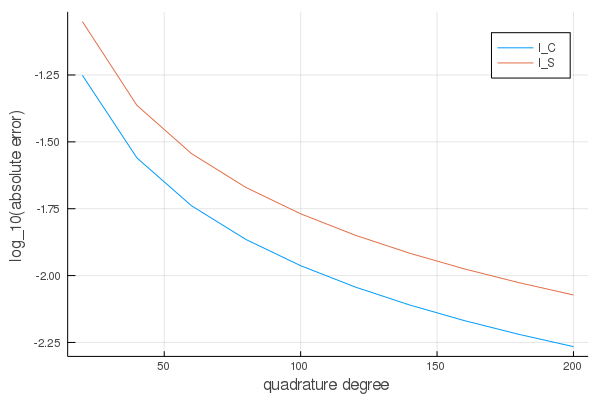
\includegraphics[scale=0.5]{WykresClogabsolute.png}
    \label{wykresC}
\end{figure}

Przedziałem (ilością węzłów) do sprawdzenia przy użyciu tej metody było 20:20:200. Wyniki uzyskane na tym przedziale są bardzo zbliżone do wyników (na tym samym przedziale) otrzymywanych za pomocą zmodyfikowanej metody trapezów.


\section*{Kwadratury Gaussa-Legendre'a}
	Wagą nazywam funkcję ciągłą, która nie jest tożsamościowo równa 0.
%\subsection*{Kwadratura} 
%Metoda całkowania numerycznego polegająca na obliczeniu wartości wyrażenia
%\[ \sum_{i=0}^n A_if(x_i) \approx \int_a^b f(x) d x \] 
%gdzie $x_0,...,x_n\in [a,b]$.

\subsection*{Kwadratura Gaussa-Legendre'a}
Kwadratura w której węzły $x_0,x_1,...,x_n$ są pierwiastkami $n+1$-szego
wielomianu ortogonalnego $w_{n+1}$ na przedziale $[a,b]$ (z wagą $p\equiv 1$), a współczynniki są równe
\[A_i=\int_a^b \prod_{j=0,j\neq i}^n \frac{x-x_j}{x_i-x_j} dx\]. O istnieniu
wystarczająco wielu pierwiastków wielomianu ortogonalnego, oraz zasadności 
takiego doboru węzłów mówią następujące twierdzenia: 
\begin{theorem}
	Jeśli niezerowa funkcja $f\in C[a,b]$ jest ortogonalna w tym przedziale z wagą $w$ względem wszystkich wielomianów klasy $\prod_{n}$, to w $(a,b)$ zmienia znak co najmniej $n+1$ razy.
\end{theorem}
\textbf{Dowód} $1\equiv w \in \prod_{n}$, więc $\int_a^b f(x)w(x)dx = 0$, co oznacza, że $f$ musi zmieniać znak co najmniej raz. Przypuśćmy, że $f$ zmienia znak tylko $r$ razy, gdzie $r\le n $. Zatem istnieją punkty $a=a_0<a_1<...<a_{r+1}=b$ takie, że w każdym z przedziałów $(a_i,a_{i+1})$ funkcja $f$ ma stały znak. Wielomian $\prod_{r}^{i=1}(x-a_i) = b(x) \in \prod_{n}$ ma tę samą własność, więc ponieważ $f$ jest niezerowa, a $f(x)b(x)$ jest ciągła to powinno być $\int_{a}^{b} f(x)b(x)w(x)dx\neq 0$, co jest sprzeczne z założeniem, że $\int_{a}^{b}f(x)b(x)w(x)dx = 0$. \newline

W szczególności wielomian $w_{n+1}$ spełnia założenia powyższego twierdzenia, więc musi mieć dokładnie $n+1$ pierwiastków jednokrotnych.

\begin{theorem}
	Jeśli węzły $x_0,x_1,...,x_n$ są zerami $n+1$-szego wielomianu ortogonalnego $w_{n+1}$ na przedziale $[a,b]$ z wagą $w$, to kwadratura o współczynnikiach
	\[A_i=\int_a^b w(x)\prod_{j=0,j\neq i}^n \frac{x-x_j}{x_i-x_j} dx\] jest dokładana dla każdego wielomianu $f\in\prod_{2n+1}$.
\end{theorem}

\textbf{Dowód} Niech $r$ będzie resztą z dzielenia wielomianu $f$ przez $w_{n+1}$: $(q,r\in \prod_{n})$\[f = qw_{n+1} + r .\] Stąd $r(x_i) = f(x_i)$. Ponieważ kwadratura Gaussa-Legendre'a jest z założenia dokładna dla wielomianów postaci $\sum_{i=0}^n B_i\prod_{j=0,j\neq i}^n \frac{x-x_j}{x_i-x_j}$, to jest dokładna dla wszystkich wielomianów z $\prod_n$. Dla takich wielomianów kwadratura oblicza dokładną wartoś całki wielomianu interpolacyjnego danego wielomianu w węzłach $x_0,x_1,...,x_n$. Ponieważ liczba użytych węzłów jest większa niż stopień wyjściowego wielomianu to otrzymany wielomian interpolacyjny jest mu równy. Ponieważ $w_{n+1}$ jest ortogonalny względem wszystkich wielomianów stopnia co najwyżej $n$,to \[\int_a^b f(x)w(x)dx = \int_a^b r(x)w(x)dx = \sum_{i=0}^n A_ir(x_i) = \sum_{i=0}^n A_if(x_i).\] 

Nie da się skonstruować kwadratury, która przy użyciu $n+1$ węzłów będzie dokładna dla wielomianów stopnia wyższego niż $2n+1$. Niech będą dane pewne $x_0,x_1,...,x_n,A_0,A_1,...,A_n$, kwadratura $Q(f) = \sum_{i=0}^n A_if(x_i)$ nie jest dokładna dla wielomianu $\prod_{i=0}^n (x-x_i)^2$. \newline

Błąd kwadratury Gaussa-Legendre'a stopnia $n$ dla funkcji $f$ jest równy \[
	\frac{2^{2n+1}(n!)^4}{(2n+1)[(2n)!]^3}f^{(2n)}(\xi) \]
dla pewnego punktu $\xi$ należącego do przedziału całkowania.

\subsection{Otrzymane wyniki}
	Kwadratury Gaussa-Legendre'a wykorzystaliśmy do obliczenia wartości całek z funkcji $Snew$ i $Cnew$ równych odpowiednio całkom $I_S,I_C$.


\begin{figure}[ht]
    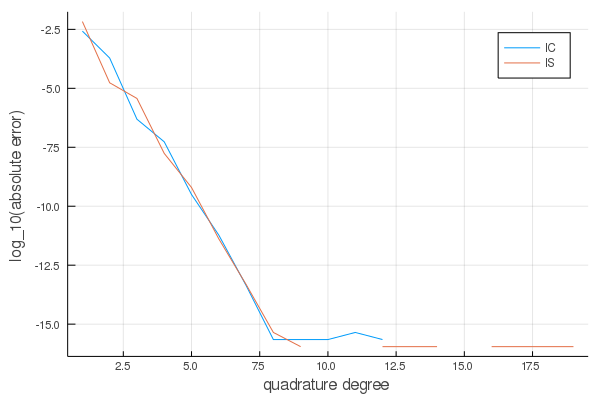
\includegraphics[scale=0.5]{WykresD1logabsolute.png}
    \label{wykresDabsolute}
\end{figure}
\begin{figure}[ht]
    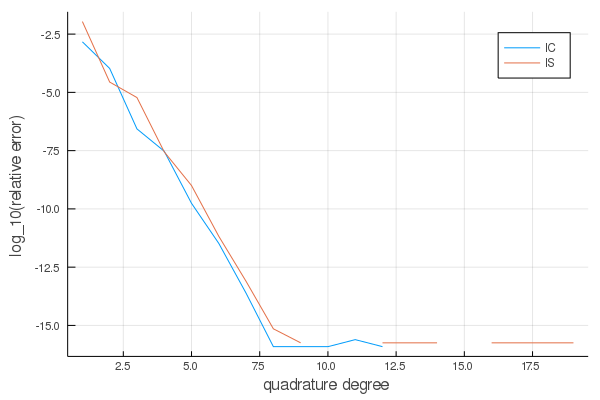
\includegraphics[scale=0.5]{WykresD1logrelative.png}
    \label{wykresDrel}
\end{figure}

\newpage
W punktach, w których wykres błędu bezwzględnego znika obliczona wartość jest równa reprezentacji wartości całki (odpowiednio $I_C$ lub $I_S$) w arytmetyce Float64. Ciąg kwadratur Gaussa-Legendre'a z funkcji ciągłej na przedziale jest zbieżny do wartości całki z tej funkcji (tw. Stieltjes'a), więc tak długo można się było spodziewać, że używanie kwadratur wyższych stopni będzie poprawiać dokładność otrzymanego wyniku, ale nawet wyniki dla bardzo niskich stopni kwadratur dają rezultaty znacznie dokładniejsze niż wcześniej użyte metody, wymagające wykonania wielokrotnie większej ilości obliczeń.

\subsection*{Złożne kwadratury Gaussa-Legendre'a}
	Dzielimy przedział $[-1,1]$ $n$ punktami równnodległymi, a następnie całkę z danej funkcji obliczamy osobno na każdym z powstałych $n-1$ przedziałów, za każdym razem stosując kwadraturę Gaussa-Legendre'a. 

\begin{figure}[ht]
    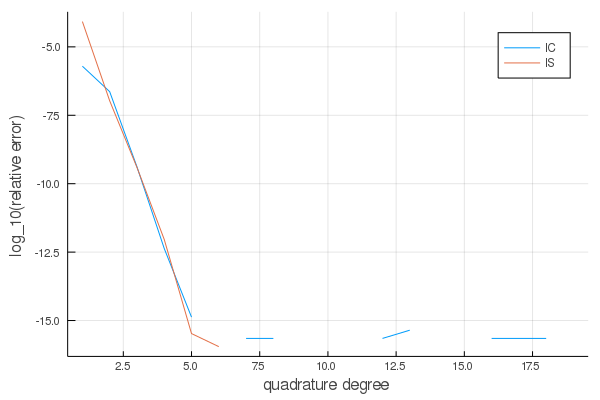
\includegraphics[scale=0.5]{WykresD2logrelative.png}
    \label{WykresD2}
\end{figure}
Powyżej widać wykres błędu względnego dla kwadratur rozbijających przedział $[-1,1]$ na trzy podprzedziały. Rozbijanie wyjściowego przedziału na większą ilość podprzedziałów nie wpływa na wyniki w sposób znaczący. Poprawia się jedynie dokładność otrzymanego wyniku dla kwadratur niższych stopni. W przypadku całki $I_C$ otrzymujemy 16 cyfr dokładnych i wynik ten nie poprawia się, nawet gdy używamy ponad 100 podprzedziałów zamiast wyjściowego $[-1,1]$. Dla 10 i więcej użytych podprzedziałów wyniki otrzymany przy obliczaniu całki $I_C$ jest dokładną wartością $I_C$ w arytmetyce Float64.  

\section*{Podsumowanie wyników}
\dots
\begin{thebibliography}{9}

  
\bibitem{kincaid}
  David Kincaid, Ward Cheney
  \emph{Analiza numeryczna - Wydawnictwo Naukowo-Techniczne, 2006}.

\bibitem{wiki}
  Wikipedia
  \emph{https://www.wikipedia.org/}.

\bibitem{pavel}
	Pavel Holoborodko - metody numeryczne
		\emph{http://www.holoborodko.com/pavel}

\bibitem{wolfram}
	Wolfram Mathworld
		\emph{http://mathworld.wolfram.com}
\end{thebibliography}


\end{document}
